\subsection{Warum agil}
Agilität im Kontext von Projektmanagement oder auch grundsätzlicher Unternehmensorganisation ist ein alternativer Ansatz für die Planung unternehmensinterner Prozesse, wie z. B. die Umsetzung eines Projekts und steht meist dem sogenannten traditionellen Ansatz gegenüber. Unter diesem traditionellen Ansatz wird für gewöhnlich der lineare Planungsprozess verstanden, welcher voraussetzt, dass Anforderungen vor der Umsetzung klar definiert und dokumentiert sind und somit Risiko minimiert wird. Diese Umstände sind allerdings nicht immer gegeben, bevor ein geplanter Prozess beginnen muss, damit Konkurrenzfähigkeit für ein Unternehmen gegeben ist. Solche zeitkritischen Prozesse sind häufig aber maßgebend für den Erfolg eines Unternehmens, wodurch ein Bedarf für eine Methode entstand, die Anpassbarkeit an sich ändernde Anforderungen und Rahmenbedingungen erlaubt \cite{agilismVsTranditionalApproaches}.

Bei traditioneller Planung erhöht sich durch diese Bedingungen das Risiko die falschen Dinge zum falschen Zeitpunkt zu tun. Agile Methodik erlaubt es diese Prozesse so effektiv wie möglich zu managen, da die Planung nicht linear, sondern iterativ stattfinde. Durch regelmäßige Feedbackschleifen mit Stakeholdern bleibt der Fokus auf Werteorientierung, da sich ändernde Anforderungen regelmäßig in den Planungsprozess der nächsten Iteration einbezogen werden. \emph{Außerdem wird die Projektverantwortung von der Rolle des Projektmanagers ins Team gegeben.} Somit entsteht eine Flexibilität und Anpassbarkeit, welche die hohe Volatilität verringert. Dadurch, dass Dinge erst dann entschieden werden, wenn es notwendig ist, ist allerdings der Gesamtaufwand und die -dauer nicht zu Beginn einschätzbar, sondern immer nur der Aufwand und die Dauer der aktuellen Iteration \cite{agilismVsTranditionalApproaches}.

Ziel bei der Wahl der Planungsmethode ist immer den Erfolg der Umsetzung des geplanten Prozesses zu maximieren. Für Projekte wird dieser Erfolg in zwei Schlüsselfaktoren unterteilt. Kurzfristiger Projekterfolg wird durch die Effizienz definiert, langfristiger Projekterfolg durch Effektivität. Diese beiden Faktoren werden durch Eingrenzung des Projektumfangs, schneller Lieferung, Qualitätssicherung, Kundenzufriedenheit und klare Kommunikation an und zwischen Stakeholdern \cite{traditionalAndAgileOnProjectSuccess}. Im Beispiel des Projektmanagements wurde bereits untersucht, inwiefern die Verwendung von agilen Methoden, den Projekt erfolgt steigert. Dabei stellte sich heraus, dass gerade der Erfolg agiler Projektplanung von der Qualität der Teamarbeit abhängig ist.
Außerdem zeigte sich, dass in den meisten Fällen ein hybrider Ansatz sowohl dem traditionellen als auch dem strikt agilen Ansatz überlegen ist \cite{traditionalAndAgileOnProjectSuccess}.
Hat ein Projekt keinen Bedarf für agile Vorgehensweisen und wird dennoch agil durchgeführt, kann dies zu Verminderung des Projekterfolgs führen.

\subsection{Agile Projektstruktur}
Um die Ziele eines agilen Ansatzes im Projektmanagement zu erreichen, muss die Struktur auch dem agilen Umsetzungsprozess gewachsen sein. Dazu muss das Projekt mit einem iterativen Gedanken geplant werden. Das Projekt muss also nicht nur als ein fertiges Produkt welches am Ende der vollständigen Umsetzung entstanden ist, sondern auch die Zwischenprodukte die am Ende jeder Iteration bereits entstanden sind, betrachtet werden. Das Ziel von agilem PM ist funktionierende Software und das so früh wie möglich, ohne das das vollständige Projekt umgesetzt werden muss. Hierzu verwendet man das Minimum Viable Product(MVP) und Minimum Marketable Features (MMF) \cite{}.  Mit diesen funktionierenden und in sich geschlossenen Iterationen kann während der Umsetzung dann regelmäßig ein Feedbackprozess stattfinden. Diese Feedbackschleifen sind essenziell für die Erhaltung von Werteorientierung und Anpassbarkeit im Verlauf des Projekts \cite{}.

Für MVP und MMF muss das Projekt bis zu einer bestimmten Granularität segmentiert werden. Hierzu verwendet man typischerweise sogenannte Epics und User-Stories. Epics sind in sich geschlossene Bestandteile des Produkts. Mehrere dieser Epics bilden zusammen mit ihrer vollständigen Umsetzung ein MVP oder MMF. Epics können anschließend in User-Stories aufgespalten werden, welche konkrete Funktionalitäten beschreiben. \cite{}

\vspace{20pt}
\begin{center}
    \begin{minipage}{0.8\linewidth}
        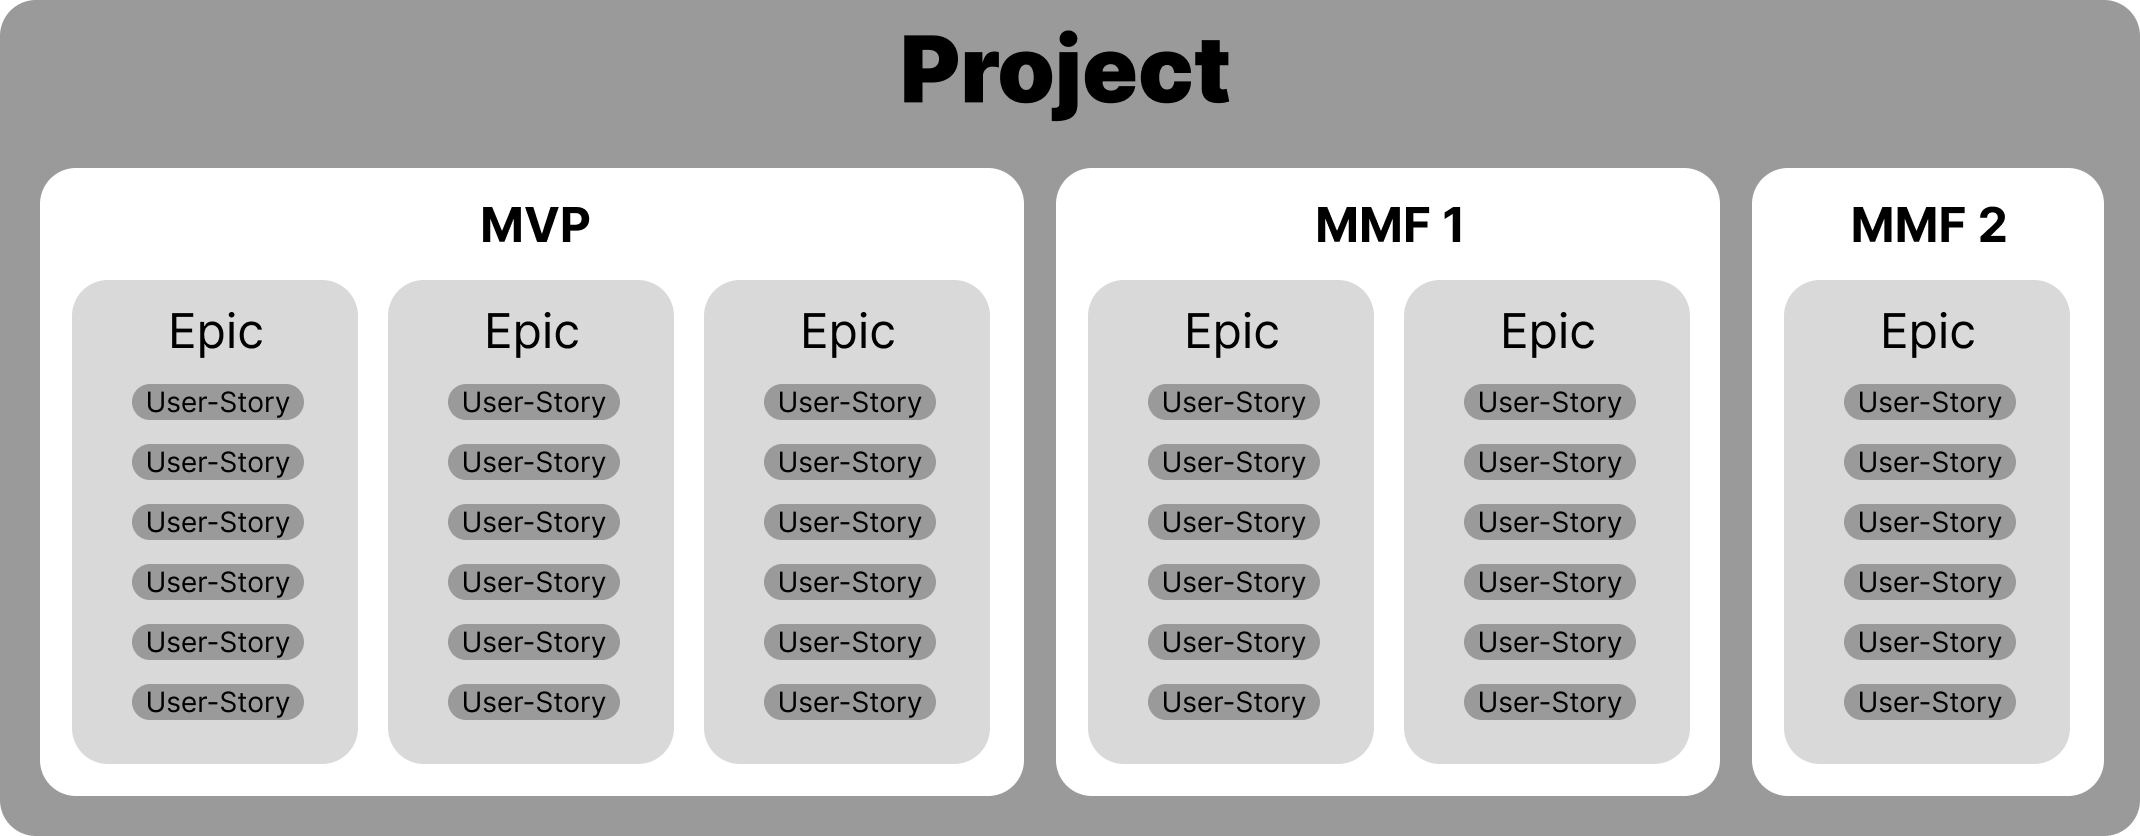
\includegraphics[width=\linewidth]{Project-Tree}
        \captionof{figure}{Agile Projektsegmentierung}
    \end{minipage}
\end{center}
\vspace{20pt}

User-Stories können zum Zeitpunkt der Umsetzung erneut in sogenannte Tasks unterteilt werden. Tasks sind Arbeitspakete die effektiv von einer einzelnen Person an einem Stück bearbeitet werden können. Diese Arbeitspakete sollten von den operativen Projektteammitgliedern definiert werden, da diese die am besten abschätzen können, wie die Beschaffenheit der Tasks sein muss, um Teamressourcen, wie Kapazität und Kompetenzen innerhalb des Teams, optimal zu nutzen. \cite{}

Für die Umsetzung gibt es verschiedene Kommunikations-Frameworks. Die beiden meist vertretenen Frameworks sind Scrum und Kanban. Beide Frameworks bieten Möglichkeiten den iterativen Umsatzprozess mit regelmäßigen Meetings, die ein konkretes Ziel verfolgen, zu strukturieren.

\subsection{Agiles Portfoliomanagement}
Der agile Ansatz kann ebenfalls für das Portfoliomanagement innerhalb eines Unternehmens verwendet werden. Traditionelles Portfoliomanagement oder auch Projekt Portfoliomanagement basiert auf … \cite{}.

Agiles Portfoliomanagement dagegen hat das Ziel Unternehmensziele mit Initiativen oder Projekten zu verknüpfen und somit den Fluss von geleisteter Arbeit auf operativer Ebene zu steuern, um diese Ziele zu erreichen und dabei die Dynamik agiler Frameworks beizubehalten. \cite{}

% In a first cross-case study comparing the application of agile portfolio man- agement in 14 large organisations to existing literature and professional frame- works, Stettina and Hörz [1] point at the characteristics of agile portfolio manage- ment as (1) transparency of resources and work items, improving trust, decision- making, and resource allocation; (2) collaboration, close collaboration based on routinised interaction and artefacts enabling frequent feedback-loops across the domains; (3) commitment to strategically managed portfolios; (4) team orientation, removing unrest in resource allocation and building capabilities in teams.

\subsection{Agile Unternehmensstrukturierung}
Kombiniert man agile Projektstruktur und agiles Portfoliomanagement kann eine Organisation Business Agilität erreichen.

\subsection{Beispiel Flight-Level}
Flight-Level ist eine von Klaus Leopold entwickelte Methode, welche eine mögliche Form von agiler Unternehmensstrukturierung bietet. Die Methode Flight-Level wird hierbei von Leopold  als Kommunikations-Framework bezeichnet und unterteilt ein Unternehmen in 3 Ebenen oder auch Flight-Level, also Flughöhen bezeichnet:
\begin{longtable}{p{3cm}p{10cm}}
    Flight-Level 1: & Operative Ebene mit einem Projekt oder Team \cr
    Flight-Level 2: & Koordinierung der Zusammenarbeit mehrerer Teams\cr
    Flight-Level 3: & Strategisches Portfoliomanagement.
\end{longtable}

Die Levels sollen einen Blick in verschiedenen Detailgraden auf das Unternehmen ermöglichen, ähnlich wie bei einem Blick aus einem Flugzeug in verschiedenen Flughöhen \cite{}. Kommunikation zwischen den Ebenen wird als kritischer Faktor dargestellt, welcher die Wertschöpfung steigern, da sich das Unternehmen besser und schnelle an die Veränderungen des Marktes anpassen können soll und somit die Konkurrenzfähigkeit bewahren kann. Ähnlich wie bei agilen Projektmanagement-Frameworks, gibt diese Methode eine klare Struktur in der Kommunikation vor.